\chapter{ಮಾಯಾ ಚೌಕದ ಕೆಲವು ವಿವರಗಳು}

ಮಾಯಾಚೌಕದ ರಚನಾವಿಧಾನವನ್ನು ಅಧ್ಯಯಿಸುವ ಮೊದಲು ಗಣಿತಶಾಸ್ತ್ರದಲ್ಲಿ ಮಾಯಾಚೌಕಕ್ಕೆ ಸಂಬಂಧಿಸಿದಂತೆ ಬಳಸಲಾಗುವ ಕೆಲವು ಪದಗಳನ್ನು ಪರಿಚಯಿಸಿಕೊಳ್ಳೋಣ.

\section*{ಮಾಯಾ ಚೌಕ :}

3 ಅಥವಾ ಅದಕ್ಕಿಂತ ಹೆಚ್ಚು ಮನೆಗಳನ್ನು ಸಾಲುಗಳಲ್ಲಿ ಹೊಂದಿರುವ ಚಚ್ಚೌಕದ (ಖಟ್ಠಿಚ್ಟಛಿ) ಮನೆಗಳಲ್ಲಿ ಸಂಖ್ಯೆಗಳನ್ನು ತುಂಬಿಸಿ. ಪ್ರತಿ ಸಾಲಿನ ಸಂಖ್ಯೆಗಳ ಮೊತ್ತ ಸ್ಥಿರಾಂಕವಾದರೆ ಅದು ಮಾಯಾಚೌಕ.
\begin{figure}[H]
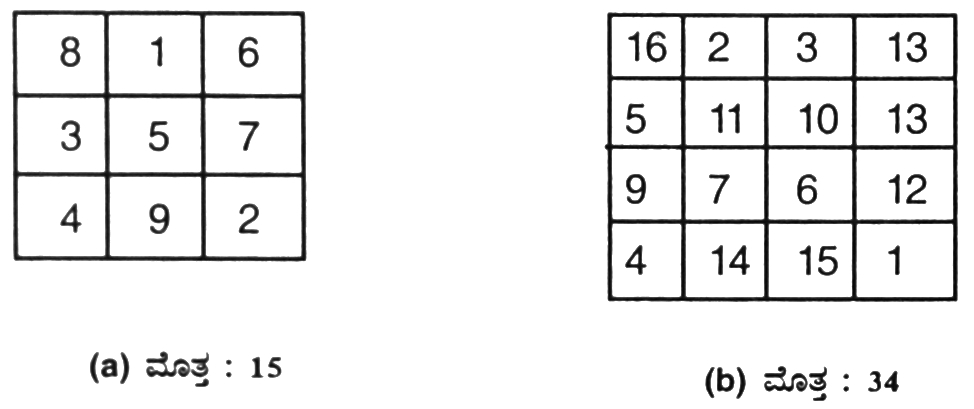
\includegraphics{src/figures/chap2/fig2-1.jpg}
\end{figure}

\section*{ಕ್ರಮವರ್ಗ : (Order)}

ಚೌಕದ ಒಂದು ಸಾಲಿನಲ್ಲಿ ಎಷ್ಟು ಮನೆಗಳಿರುತ್ತದೆಯೋ ಅದು ಮಾಯಾಚೌಕದ ಕ್ರಮವರ್ಗವನ್ನು (Order) ಸೂಚಿಸುತ್ತದೆ.

(a) ಯು 3ನೇ ಕ್ರಮವರ್ಗ, (b) ಯು 4ನೇ ಕ್ರಮವರ್ಗ

\{ X$^2$ ನ್ನು $X$ನ ವರ್ಗ  X-Squared ಎಂದು ಬೀಜಗಣಿತದಲ್ಲಿದೆ. ಮಾಯಾಚೌಕಕ್ಕೆ ಸಂಬಂಧಿಸಿದಂತೆ ಬಳಸುವ ಕ್ರಮವರ್ಗ (Order) ನ್ನು ‘‘ವರ್ಗ’’ (Square) ಎಂದು ಗ್ರಹಿಸಬಾರದು. \}

ಅಡ್ಡಸಾಲುಗಳು ಮತ್ತು ಕಂಭಸಾಲುಗಳು.
\begin{figure}[H]
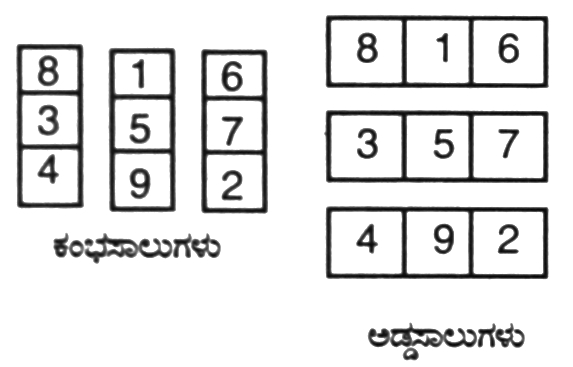
\includegraphics{src/figures/chap2/fig2-2.jpg}
\end{figure}

ಮಾಯಾಚೌಕವನ್ನು ಮೇಲಿನಿಂದ ಕೆಳಕ್ಕೆ ಸೀಳಿದಾಗ ಬರುವುದು ಕಂಭಸಾಲುಗಳು.

ಮಾಯಾಚೌಕವನ್ನು ಅಡ್ಡಲಾಗಿ ಸೀಳಿದಾಗ ಬರುವುದು ಅಡ್ಡಸಾಲುಗಳು.

ಮಾಯಾಚೌಕದ ಕ್ರಮವರ್ಗ (Order) ದಷ್ಟೇ ಸಂಖ್ಯೆಯ ಸಾಲುಗಳು ಇರುತ್ತವೆ.

ಕರ್ಣಗಳು ಮತ್ತು ಉಪಕರ್ಣಗಳು

ಮಾಯಾಚೌಕದ ಒಂದು ಮೂಲೆಯಿಂದ ಎದುರು ಮೂಲೆಗೆ ಇರುವ ಸಂಖ್ಯೆಗಳ ಸಾಲಿಗೆ ಕರ್ಣಗಳು ಎನ್ನಲಾಗಿದೆ. ಯಾವುದೇ ಮಾಯಾ ಚೌಕದಲ್ಲಿ ಎರಡು ಕರ್ಣಗಳು ಇರುವುವು.
\begin{figure}[H]
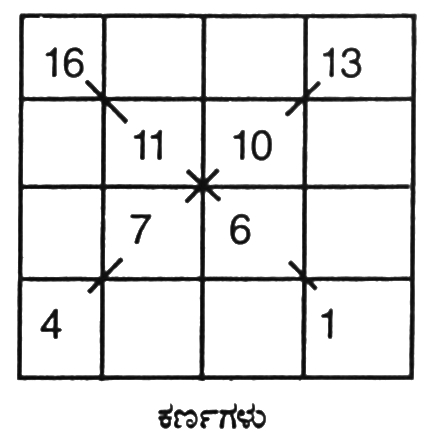
\includegraphics{src/figures/chap2/fig2-3.jpg}
\end{figure}

ಕರ್ಣಗಳನ್ನು ಹೊರತುಪಡಿಸಿ ಉಳಿದಂತೆ ಮನೆಗಳನ್ನು ಓರೆಯಾಗಿ ತೆಗೆದುಕೊಂಡರೆ, ಉಪಕರ್ಣಗಳು ಲಭಿಸುತ್ತವೆ. (Short Diagonals)
\begin{figure}[H]
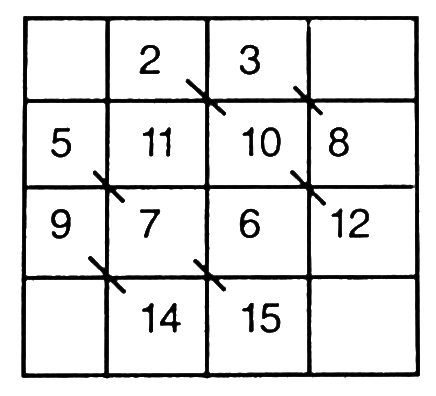
\includegraphics{src/figures/chap2/fig2-4.jpg}
\end{figure}

9,14;5,7,15;2,10,12; 3,8 ಇವು ಉಪಕರ್ಣಗಳು

ಹೀಗೆಯೇ, 5,2;9,11,3; 14,6,8;15,12ಇವೂ ಉಪಕರ್ಣಗಳು.

\section*{ಮೊತ್ತ ಅಥವಾ ಮಾಯಾ ಸ್ಥಿರಾಂಕ (Magic Constant)}

ಯಾವುದೇ ಅಡ್ಡಸಾಲಿನ, ಕಂಭಸಾಲಿನ ಅಥವಾ ಕರ್ಣಗಳಲ್ಲಿನ ಸಂಖ್ಯೆಗಳ ಮೊತ್ತವನ್ನು ‘‘ಮಾಯಾಚೌಕದ ಮೊತ್ತ’’ ಅಥವಾ ‘‘ಮಾಯಾಸ್ಥಿರಾಂಕ’’ ಎನ್ನಲಾಗಿದೆ. ಸಾಮಾನ್ಯವಾಗಿ ಇದನ್ನು ‘‘ಮೊತ್ತ’’ ಎಂದು ಕರೆಯಲಾಗುತ್ತದೆ.
\begin{figure}[H]
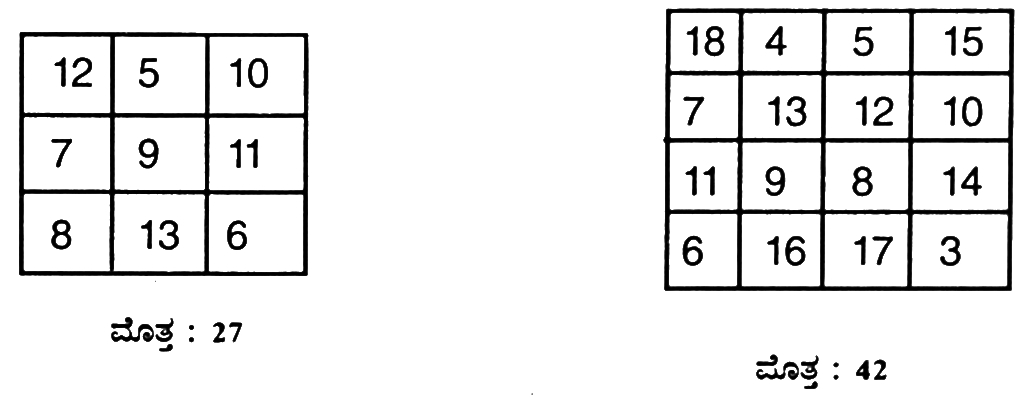
\includegraphics{src/figures/chap2/fig2-5.jpg}
\end{figure}
